\section{
  Dusty vertical shear instability}\label{results} 

When $\tstop=0$ we may construct exact dusty equilibra by specifying
the dust-to-gas ratio, as described in \S\ref{eqm}. We use this to
examine the effect of dust on classic VSI, defined to be driven by the
temperature gradient (\S\ref{dusty_vsi_int}). For simplicity we
consider constant input values of the midplane dust-to-gas ratio
$\epsilon_0$ and the characteristic dust thickness $\Hd$. These,
together with the perturbation wavenumber $k$, comprises main the
parameters of the linear problem. We fix the radial power-law index
for the midplane gas density to $p = -1.5$, that for the
temperature profile to $q=-1$; and set the gas disk aspect-ratio
$h_\mathrm{g}=0.05$. These are fiducial values used in \citetalias{lin15}. 


\subsection{Qualitative expectations}
\citetalias{lin15} find the appropriate way to compare 
destabilizing vertical shear to stabilizing vertical buoyancy is
$r\p_z\Omega/\OmK$ against $N_z^2/\OmK^2$. We see from \S\ref{vertshear}
and \S\ref{vbuoyancy} that $|r\p_z\Omega|\sim q h_\mathrm{g}\OmK$ for a
thin, gas dominated disk; while $N_z^2\sim \epsilon\OmK^2$. Thus we
expect dust-induced buoyancy forces to stabilize the disk against the
VSI where $\epsilon \gtrsim h_\mathrm{g}$. 

%\begin{align}

\subsection{Effect of dust-loading}
We first vary the midplane dust-to-gas ratio 
$\epsilon_0\in[10^{-3},1]$, fixing the dust thickness to 
$\Hd=0.99\Hg$. Then  $\epsilon$ is roughly constant with height. We
set the vertical domain to $\zmax=5\Hg$.  

We compare in Fig. \ref{compare_vshear_fixHd} the basic state
vertical shear rate, which is destabilizing, and the vertical buoyancy
frequency, which is stabilizing. For the nearly dust-free disk
$\epsilon_0=10^{-3}$ the vertical shear dominates buoyancy for all
$|z|>0$. However, a heavy dust-load with $\epsilon_0=1$ renders the
buoyancy to dominate over vertical shear in the disk atmosphere
$|z|\gtrsim 2.5$. We thus expect instability all heights for
$\epsilon_0=10^{-3}$, but to be restricted to the midplane for
$\epsilon_0=1$. 

\begin{figure}
  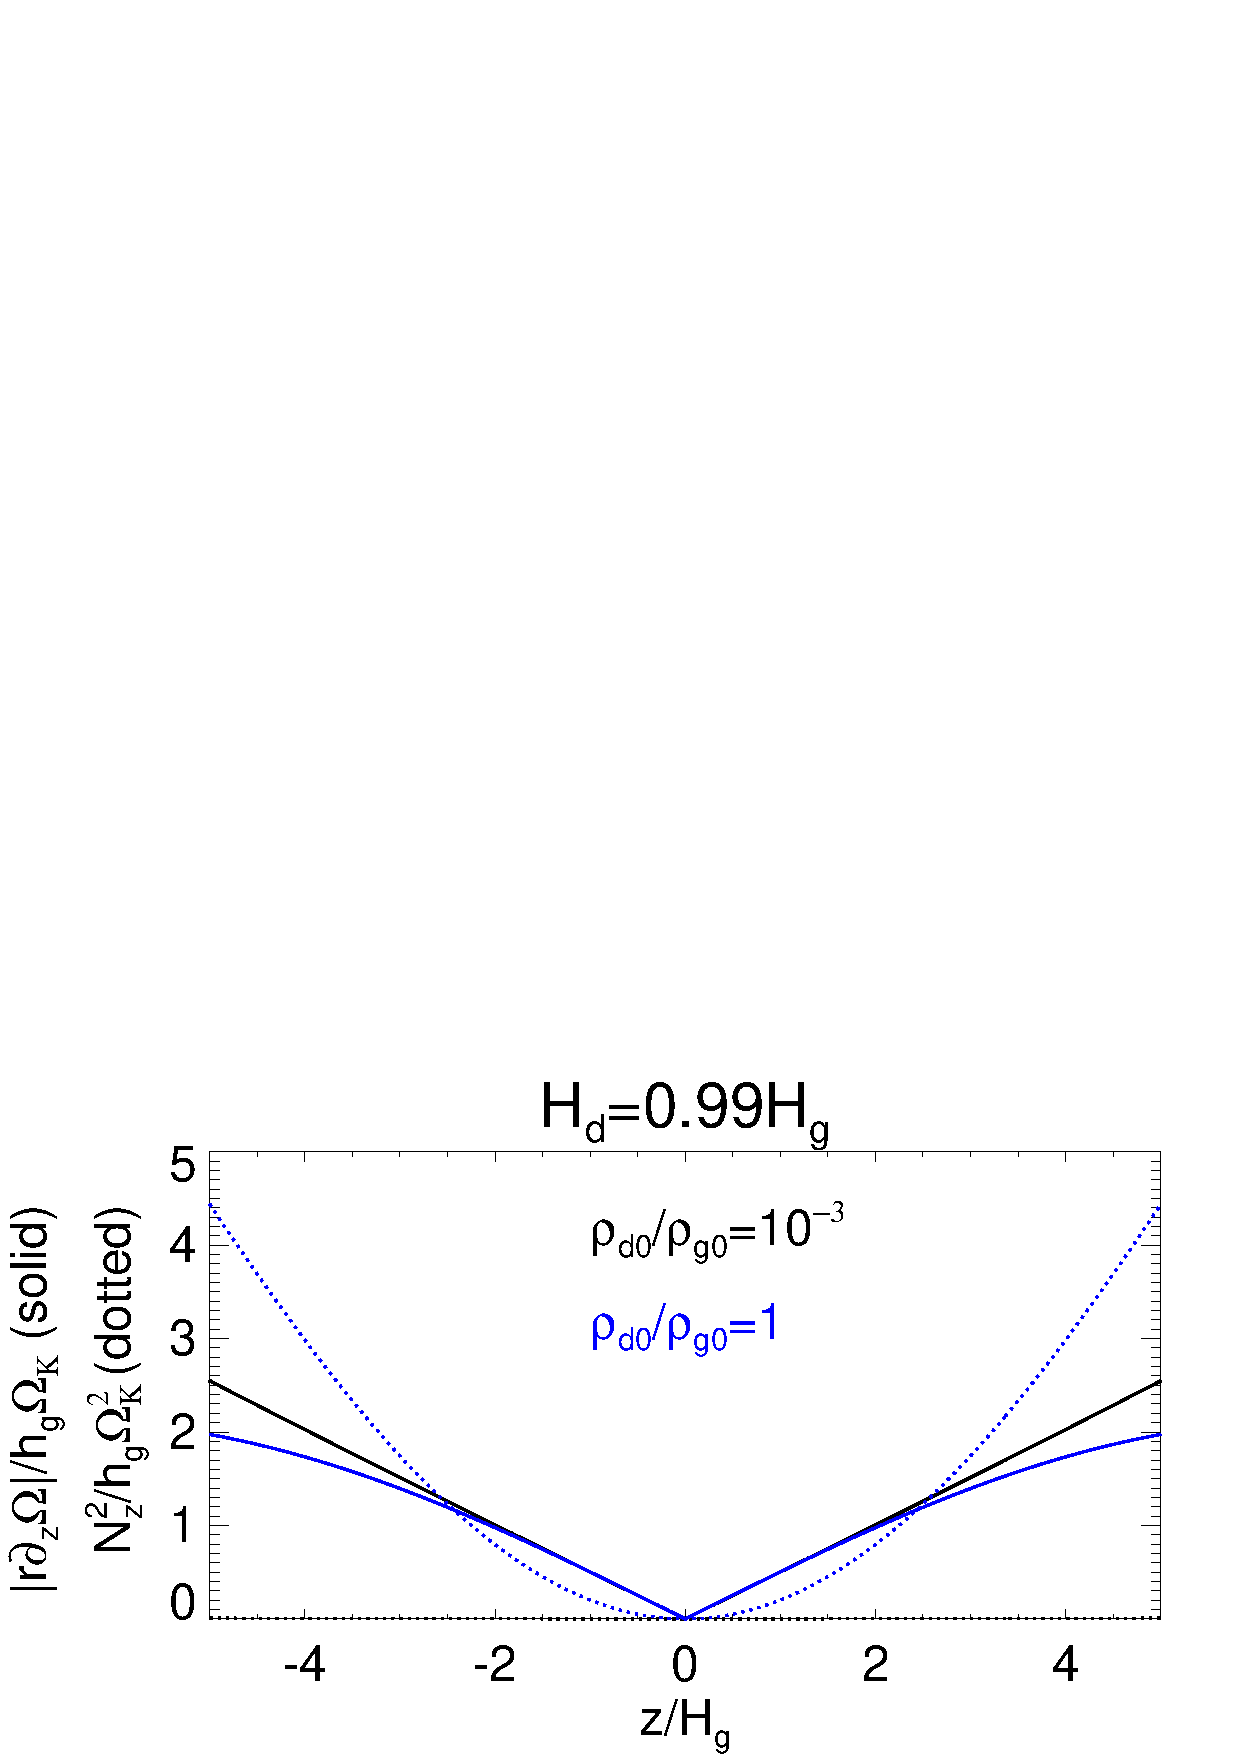
\includegraphics[width=\linewidth]{figures/compare_vshear_Nz2_fixHd} 
  \caption{Vertical shear rate (solid) compared to vertical buoyancy
    (dotted) in a locally isothermal, dusty disl with midplane dust-to-gas ratio
    of $\epsilon_0=10^{-3}$ (black) and $\epsilon_0=1$ (blue). 
    The dust layer thickness is fixed to $\Hd=0.99\Hg$ so the 
    dust-to-gas ratio $\epsilon$ is approximately constant with
    height. 
    \label{compare_vshear_fixHd}
    }
\end{figure}

Fig. \ref{vsi_dust_loading} show unstable modes for different values
of $\epsilon_0$ with fixed perturbation wavenumber  $k\Hg = 30$. The
eigenvalue distributions for $\epsilon_0 \leq 10^{-2}$ are similar to the
dust-free fiducial case considered by \citetalias{lin15}, consisting
of the roughly horizontal `body modes' and the nearly-vertical
`surface modes'. The latter is due to the imposed vertical boundaries
\citep{barker15}.  

We find that increasing the dust-to-gas ratio reduce VSI growth
rates. Notably `surface modes', which are typically fastest growing in
the dust-free case, are surpressed in dusty disks for $\epsilon_0\geq
0.1$. The body modes' growth rates remain $\sim O(h_\mathrm{g}\OmK)$
but their oscillation frequency increases with
$\epsilon_0$. The total number of modes do not change
significantly. This is in contrast with the effect of increasing
cooling times, where \citetalias{lin15} find fewer unstable modes.
%until the system is eventually completely stable. 

\begin{figure}
  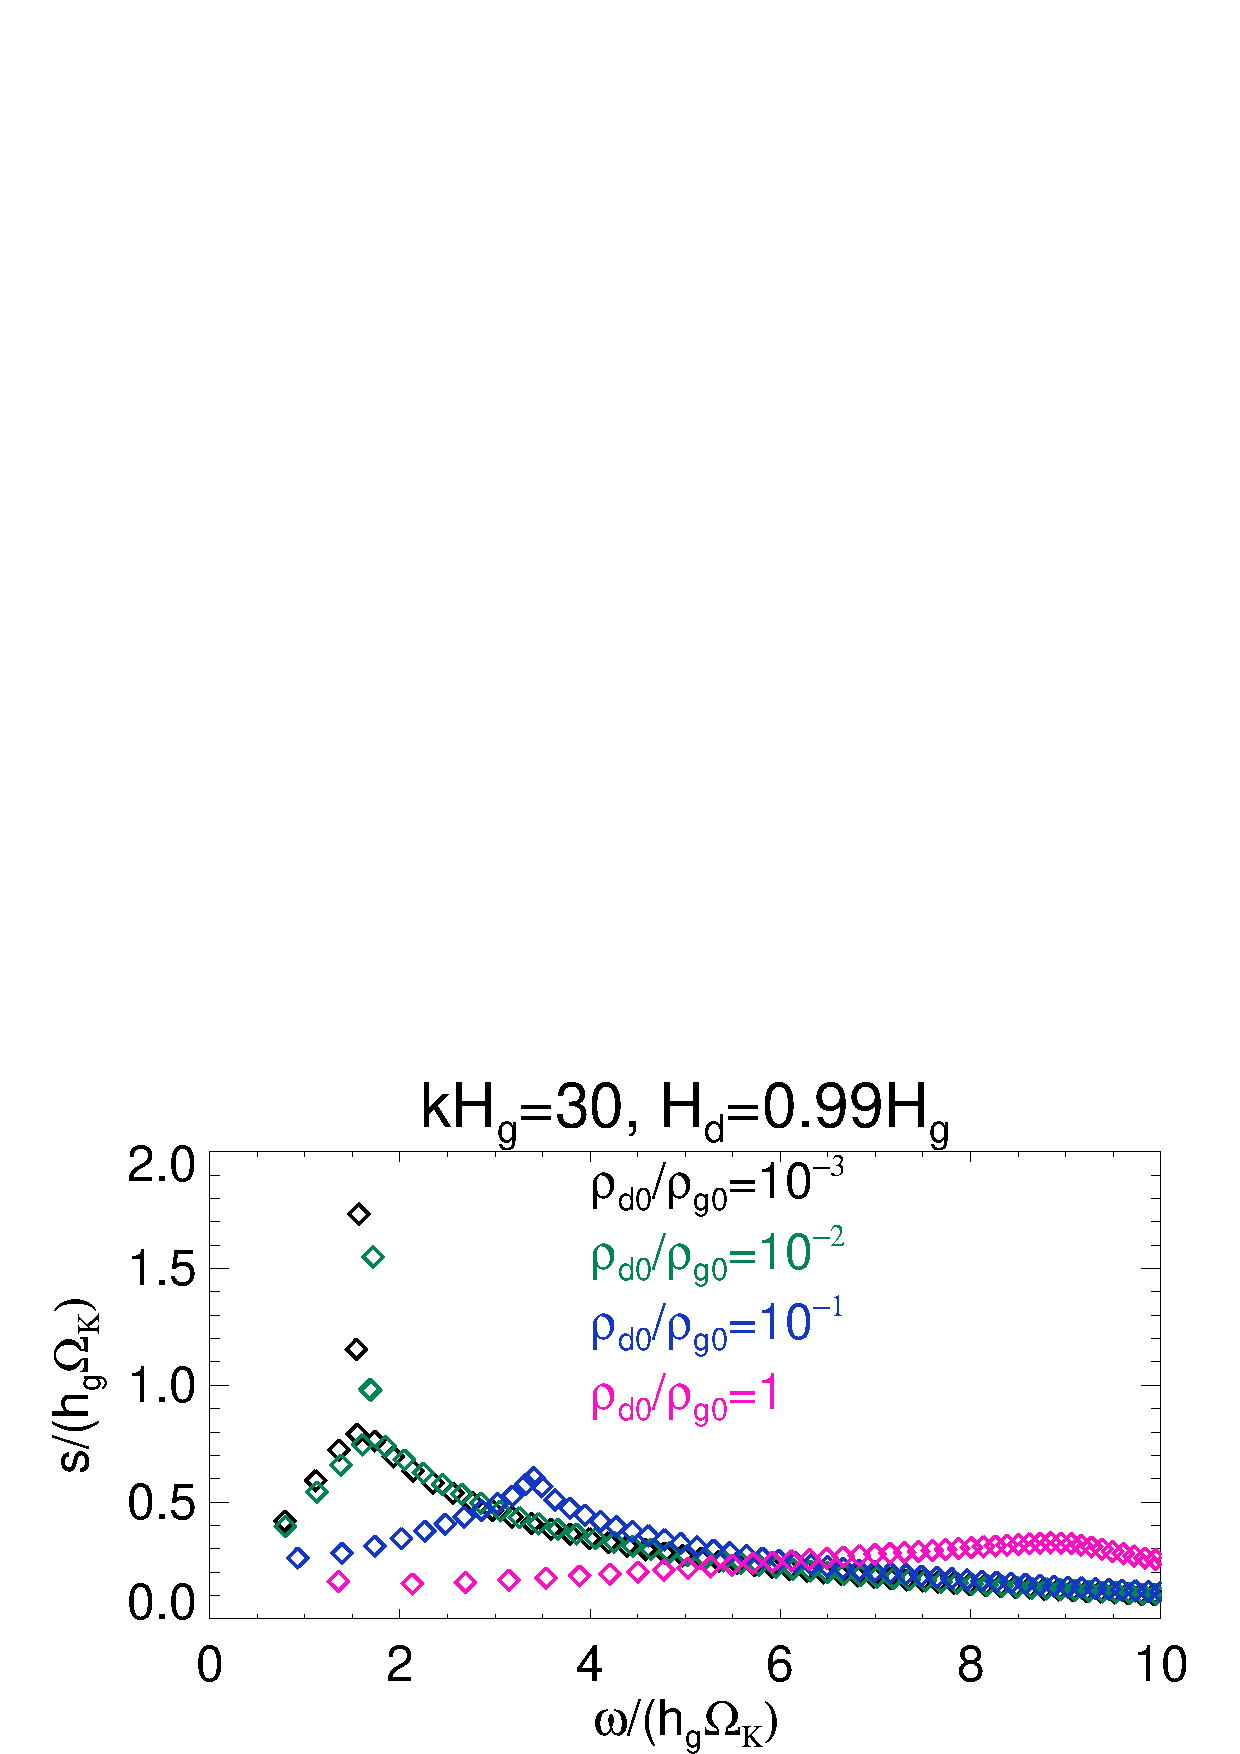
\includegraphics[width=\linewidth]{figures/compare_eigenvals_kx30Hd1} 
  \caption{Unstable modes in a locally isothermal, perfectly coupled
    dusty disk with fiducial parameters
    $(p,q,h_\mathrm{g}, \Hd/\Hg )=(-1.5,-1,0.05, 0.99)$. The real
    frequency $\omega$ and growth rates $s$ are shown for a range of
    midplane dust-to-gas ratios $\epsilon_0=\rho_\mathrm{g0}/\rho_\mathrm{d0}$. 
    \label{vsi_dust_loading}
    }
\end{figure}

The lowest frequency `fundamental' body mode is energetically dominant
because the entire disk column is perturbed \citep[cf. surface modes
  which only disturb the disk boundaries,][]{umurhan16c}. In Fig. \ref{vsi_dust_loading2d}
we compare the fundamental mode between the nearly 
dust-free case $\epsilon_0=10^{-3}$ an a dusty disk with
$\epsilon_0=1$. Dust-loading preferentially
stabilizes the disk atmosphere against the VSI, restricting
meridional motions to $|z|\lesssim 2\Hg$, where most of the disk mass
reside. This is consistent with the above comparison of the basic state vertical
shear and buoyancy. Notice also the perturbed dust-to-gas ratio,
$\delta\epsilon$, shifts from being maximized at the disk boundaries
to the midplane. 

\begin{figure}
%  \includegraphics[scale=0.54, clip=true, trim=0cm 2.5cm 0cm 0cm]{figures/result2d_dg1d-3.ps}\\
%  \includegraphics[scale=0.54]{figures/result2d_dg1.ps} 
\includegraphics[scale=0.32, clip=true, trim=0.5cm 0cm 3cm 0cm]{figures/result2d_dg1d-3.ps}\includegraphics[scale=0.32, clip=true, trim=1.8cm 0cm 0cm 0cm]{figures/result2d_dg1.ps}
  \caption{Fundamental dusty VSI mode in real space for midplane dust-to-gas
    ratio $\epsilon_0=10^{-3}$ (left) and $\epsilon_0=1$
    (right). The color scale shows the perturbation to the
    dust-to-gas ratio, $\delta\epsilon$; and the arrows show
    $\sqrt{\rho}\left(\dd v_x, \dd v_z\right)$. 
    \label{vsi_dust_loading2d}
    }
\end{figure}






In Fig. \ref{vsi_dust_loading_vareps} we plot the growth rates as a
function of $\epsilon_0$ for different perturbation wavenumbers $k$. We
find that dust-loading stabilizes the VSI more effectively for shorter
wavelength perturbations. This is because for high wavenumbers the
dominant modes are surface modes, which are stabilized by
dust-loading. The figure suggest that VSI becomes much less efficient
for $\epsilon_0\gtrsim 0.1$ and $k\Hg\gtrsim 50$. 

\begin{figure}
  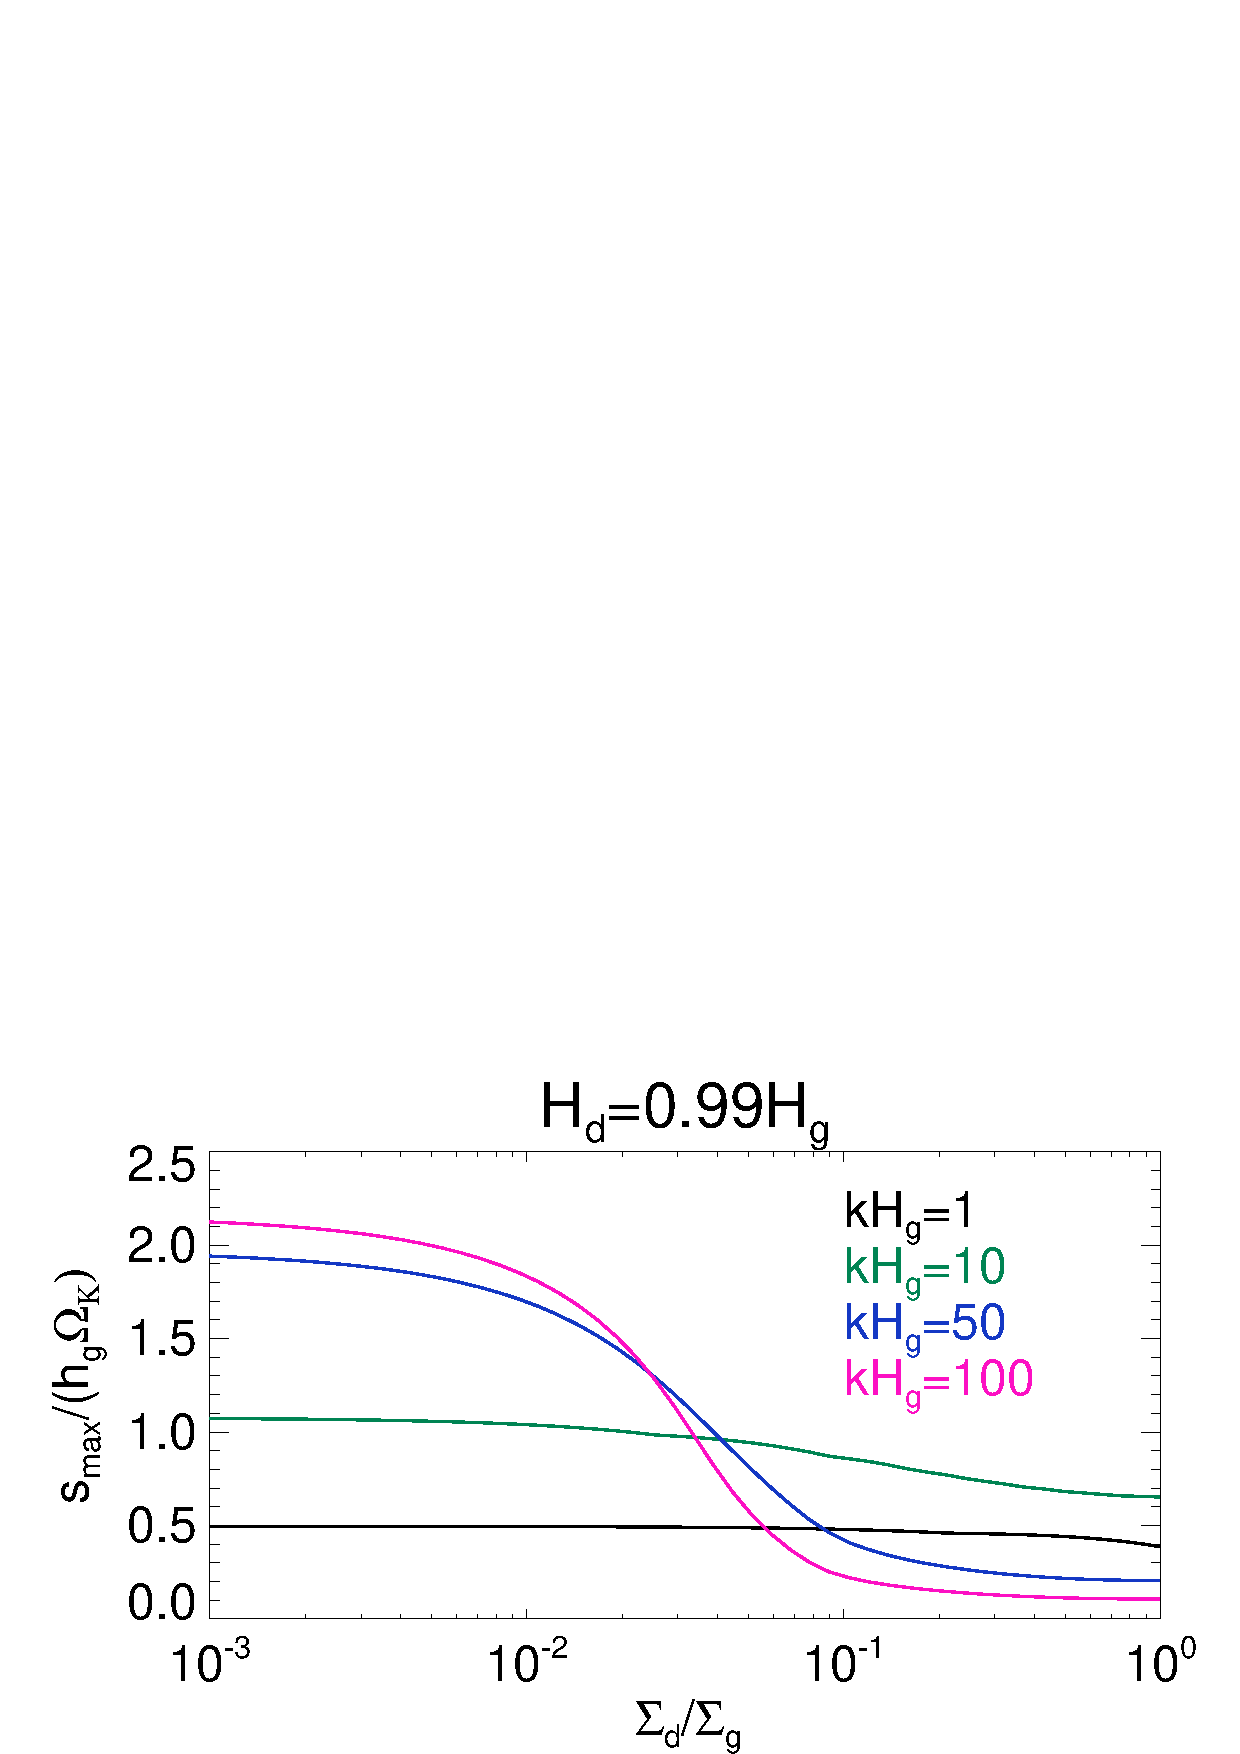
\includegraphics[width=\linewidth]{figures/compare_eigenvals_vareps2} 
  \caption{Maximum growth rate of the dusty VSI as a function of the
    midplane dust-to-gas ratio $\epsilon_0$ for perturbations with
    different radial wavenumbers $k$. The dust layer thickness is
    fixed to $\Hd\simeq \Hg$. 
    \label{vsi_dust_loading_vareps}
    }
\end{figure}

\subsection{Effect of dust thickness} 
We now vary the dust layer thickness $\Hd$ but fix the metalicity 
$Z \equiv \epsilon_0 \Hd/\Hg = \text{constant}$. This then gives the
required midplane dust-to-gas ratio. Since we will consider thin dust
layers, here we use a smaller 
domain with $\zmax=2\Hg$ so that $\epsilon$ does not become
too small. 

We set $Z=0.03$ and analyse two disks with $\Hd=0.1\Hg$ and 
$\Hd=0.99\Hg$. Fig. \ref{compare_vshear_fixZ} compares the vertical
vhear rate and buoyancy frequency. For $|z|\gtrsim 0.4\Hg$ the two
disks have the same profile with vertical shear dominating over
buoyancy. We thus expect instabilities away from the disk midplane in 
both cases. For $|z|\lesssim 0.4\Hg$, a thin dust 
layer with $\Hd=0.1\Hg$ boosts the vertical shear rate, but the
associated buoyancy is larger still. Thus we expect the mid-plane of
the disk with $\Hd=0.1\Hg$ to be stable.  

\begin{figure}
  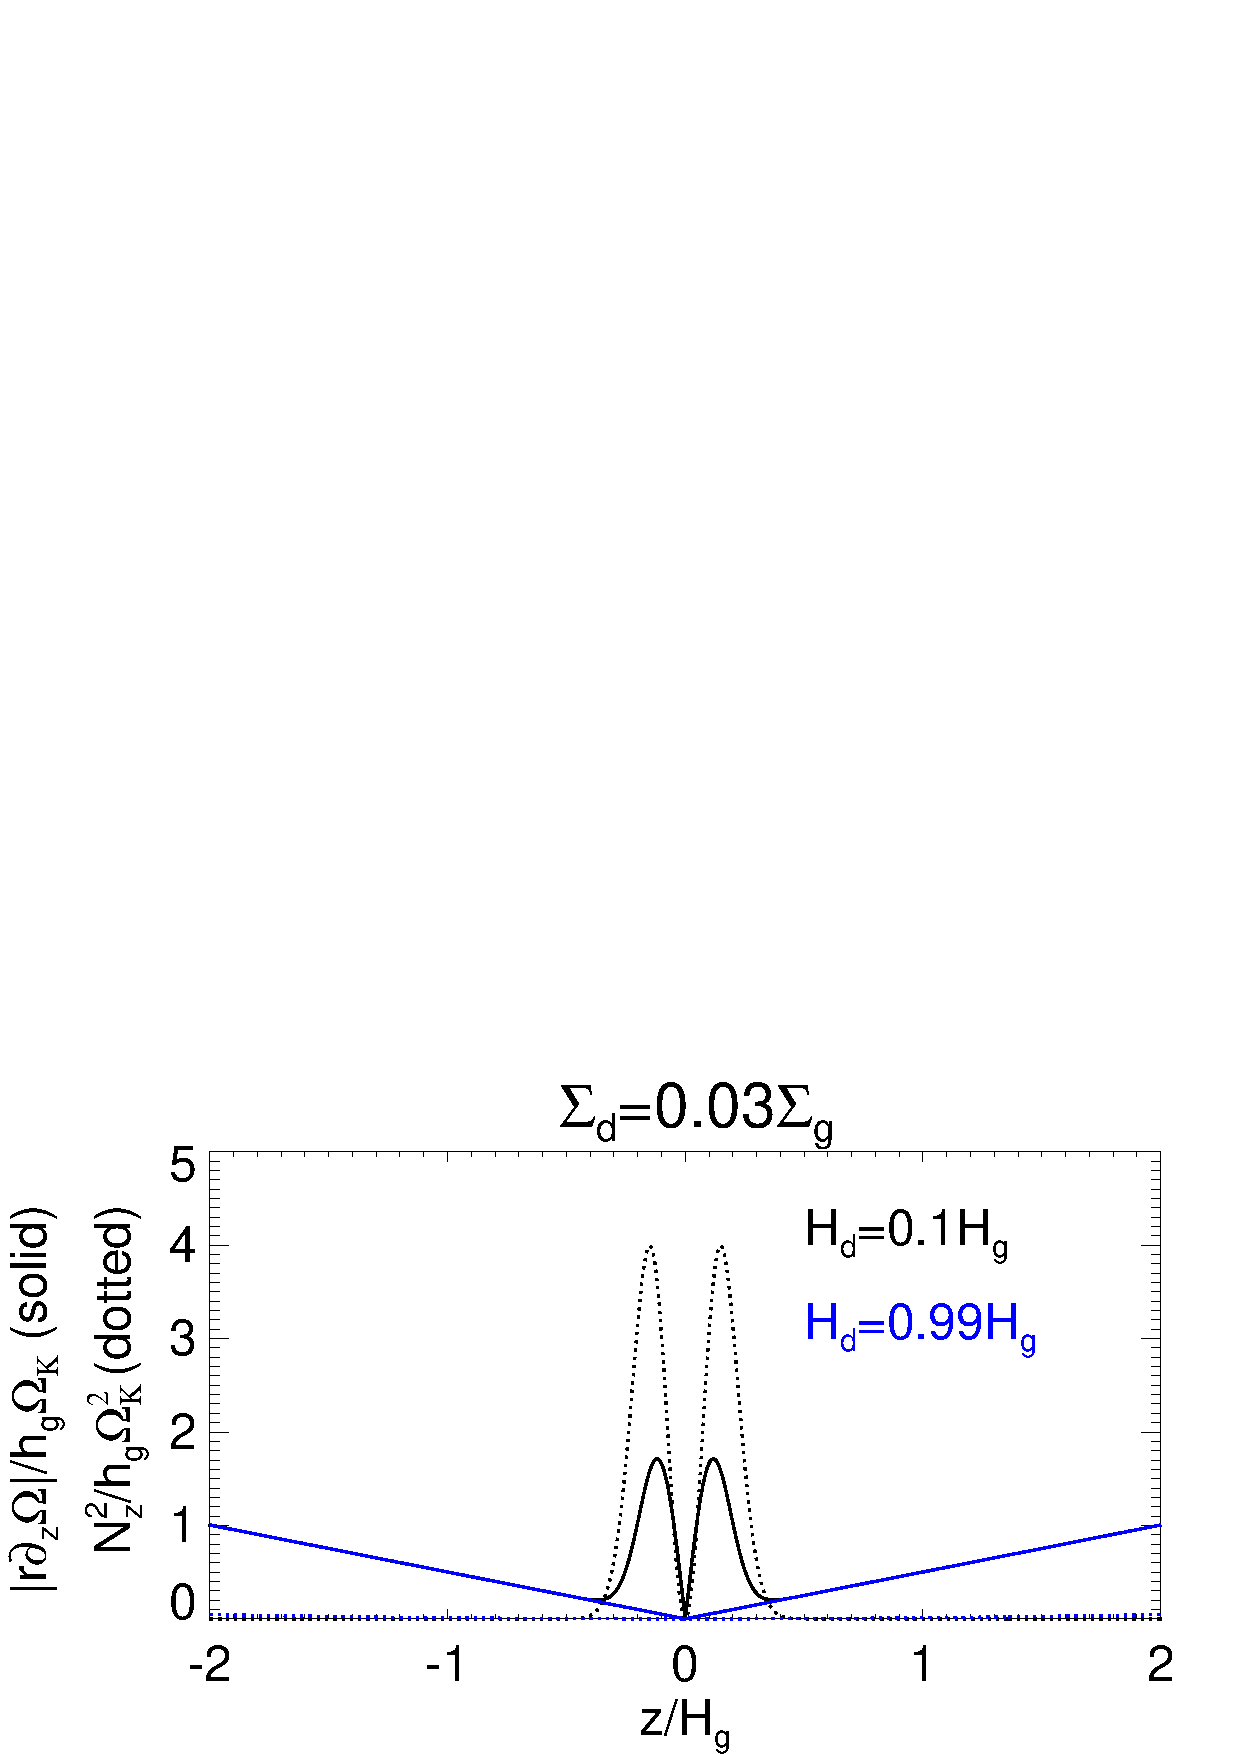
\includegraphics[width=\linewidth]{figures/compare_vshear_Nz2_fixZ} 
  \caption{Vertical shear rate (solid) compared to vertical buoyancy
    (dotted) in a locally isothermal, dusty disk 
    with metalicity $Z=0.03$ and dust thickness $\Hd=0.1\Hg$
    (black) and $\Hd=0.99\Hg$ (blue). 
    \label{compare_vshear_fixZ}
    }
\end{figure}

Fig. \ref{result2d_fixZ} compares the fastest-growing VSI body modes  
with $k\Hg=30$ for the two cases above.\citepalias[The thinner domain
  adopted here eliminates surface modes, ][]{lin15}.   
We find very similar mode 
frequencies 
\begin{align*}
  \sigma = \begin{cases}
    \left(0.3053\ii - 0.8142\right)h_\mathrm{g}\OmK & \Hd=0.99\Hg, \\
    \left(0.3178\ii - 1.2237\right)h_\mathrm{g}\OmK & \Hd=0.1\Hg,
  \end{cases}
\end{align*}
since the vertical shear profile is similar throughout most of the
disk. However, meridional motions are surpressed near the midplane of
the $\Hd=0.1\Hg$ disk, as expected from the larger buoyancy frequency
as compared to vertical shear there. This leads to a structure
analogous to PPD dead zones: a quiescent midplane between active
surface layers \citep{gammie96}.  


\begin{figure}
  \includegraphics[scale=0.32, clip=true, trim=0.5cm 0cm 3cm 0cm]{figures/result2d_Hd1.ps}\includegraphics[scale=0.32, clip=true, trim=1.8cm 0cm 0cm 0cm]{figures/result2d_Hd0d1.ps} 
  \caption{Fastest-growing dusty VSI mode in real space for midplane
    dust layer thickness $\Hd=0.99\Hg$ (left) and $\Hd=0.1\Hg$
    (right). The dust content is fixed to
    $\Sigma_\mathrm{d}=0.03\Sigma_\mathrm{g}$. 
    The color scale shows the perturbation to the
    dust-to-gas ratio, $\delta\epsilon$; and the arrows show
    $\sqrt{\rho}\left(\dd v_x, \dd v_z\right)$.
    \label{result2d_fixZ}
    }
\end{figure}

Fig. \ref{compare_eigenvals_fixZ} shows the maximum VSI growth rates
as a function of the dust layer thickness. As before, we find growth
rates are most affected by the vertical structure of the dust layer
when the perturbation wavenumer is large. VSI growth rates converge as
$\Hd\to 0$. %to dust free values?    
Thus a thin dust layer, however large its associated vertical shear,
does not affect the VSI. The non-monotonic behavior for $\Hd\gtrsim
0.5\Hg$ arises because the vertical buoyancy frequency 
\begin{align*}
N_z^2(H_d;z,Z) \simeq &Z\Hg z^2
\exp{\left(-\frac{z^2}{2\Hg^2}\right)}\OmK^2\notag\\
&\times 
\frac{1}{\Hd}\left(\frac{1}{\Hd^2} -
\frac{1}{\Hg^2}\right)\exp{\left(-\frac{z^2}{2\Hd^2}\right)}  
\end{align*}
is a non-monotonic function of $\Hd$ at fixed $z$. At $z=\Hg$ and $z=2\Hg$
the buoyancy frequency is maximized for $\Hd\simeq0.5\Hg$ and
$\Hd\simeq 0.8\Hg$, respectively. This is consistent with the abscissa
of minima in growth rates in Fig. \ref{compare_eigenvals_fixZ}. 

\begin{figure}
  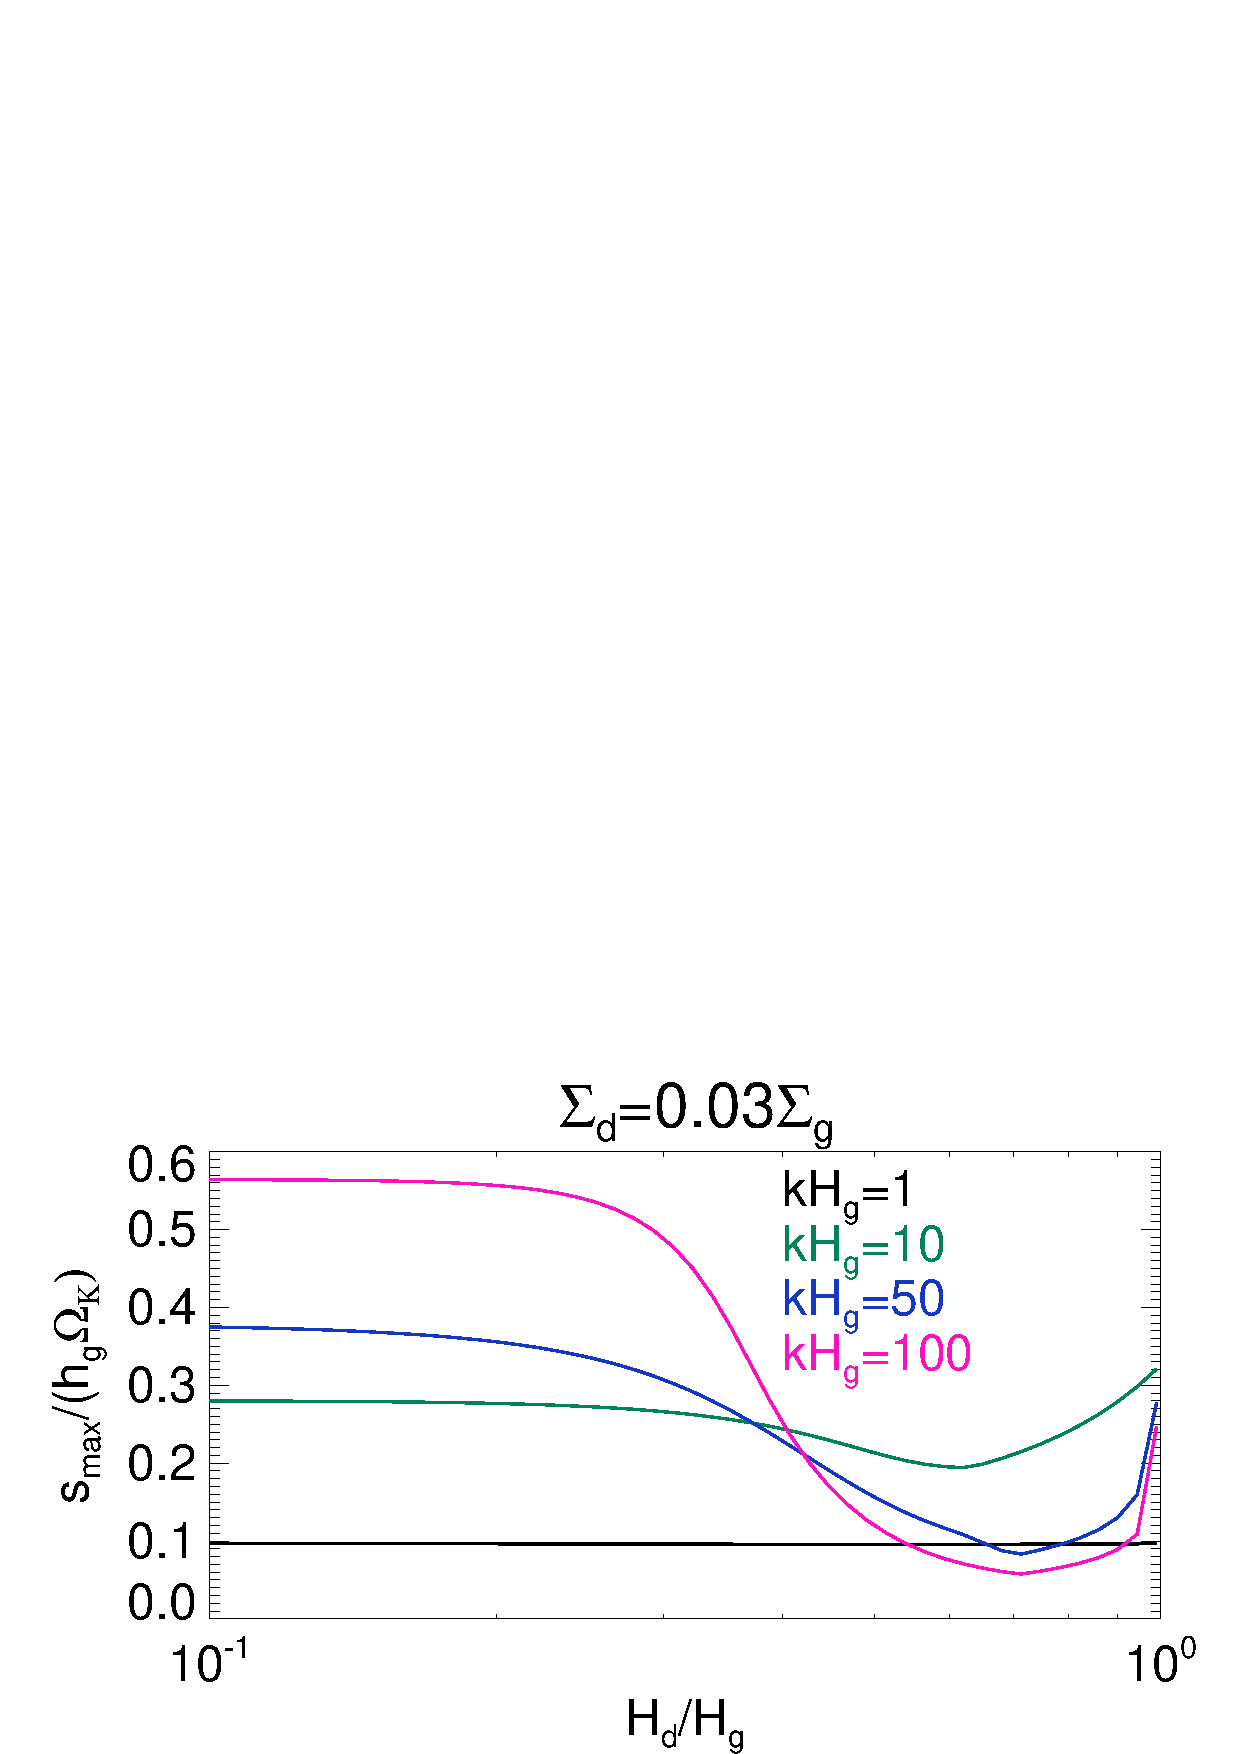
\includegraphics[width=\linewidth]{figures/compare_eigenvals_fixZ} 
  \caption{Maximum VSI growth rate for different perturbation
    wavenumbers $k$ as a function of the dust layer
    thickness $\Hd$ at fixed metalicity $Z=0.03$. 
    \label{compare_eigenvals_fixZ}
    }
\end{figure}

\subsection{Validity}
We have considered $\tstop=0$ for simplicity. When $\tstop\neq0$, a 
disk initialized as in \S\ref{eqm} will evolve 
due to dust-gas relative drift. In particular, in the
absence of turbulent/diffusive processes, dust particles settle to the
midplane on a timescale $t_\mathrm{settle}\OmK \sim 1/\tstop\OmK$
\citep{takeuchi02}. For the previous results to be valid (i.e. the
basic state does not evolve significantly) we require VSI growth
timescales $t_\mathrm{grow}\ll t_\mathrm{settle}$. Since the maximum
VSI growth rate is $\sim h_\mathrm{g}\OmK$, we need stopping times
such that 
\begin{align}
  \tstop\OmK \ll h_\mathrm{g}. 
\end{align} 
For thin PPD with $h_\mathrm{g}\sim 0.05$, our dusty VSI results are
valid for $\tstop\OmK < O(10^{-2})$.  
